\documentclass[11pt,a4paper]{article}

\usepackage[utf8]{inputenc}
\usepackage[T1]{fontenc}
\usepackage[spanish]{babel}
\usepackage[margin=1.5cm, top=1.5cm, bottom=1.5cm]{geometry}
\usepackage{graphicx}
\graphicspath{{../../01_Propuesta/Logos/}{./}}
\usepackage{fancyhdr}
\usepackage{xcolor}
\usepackage[hidelinks]{hyperref}

\definecolor{verdeosc}{RGB}{26,107,60}
\definecolor{verdemid}{RGB}{46,139,87}

\setlength{\headheight}{35pt}
\pagestyle{fancy}
\fancyhf{}
\fancyhead[L]{%
  \begin{tabular*}{\textwidth}{@{\extracolsep{\fill}}ccc@{}}
    
\includegraphics[height=0.8cm]{logo_unisucre.png} &
    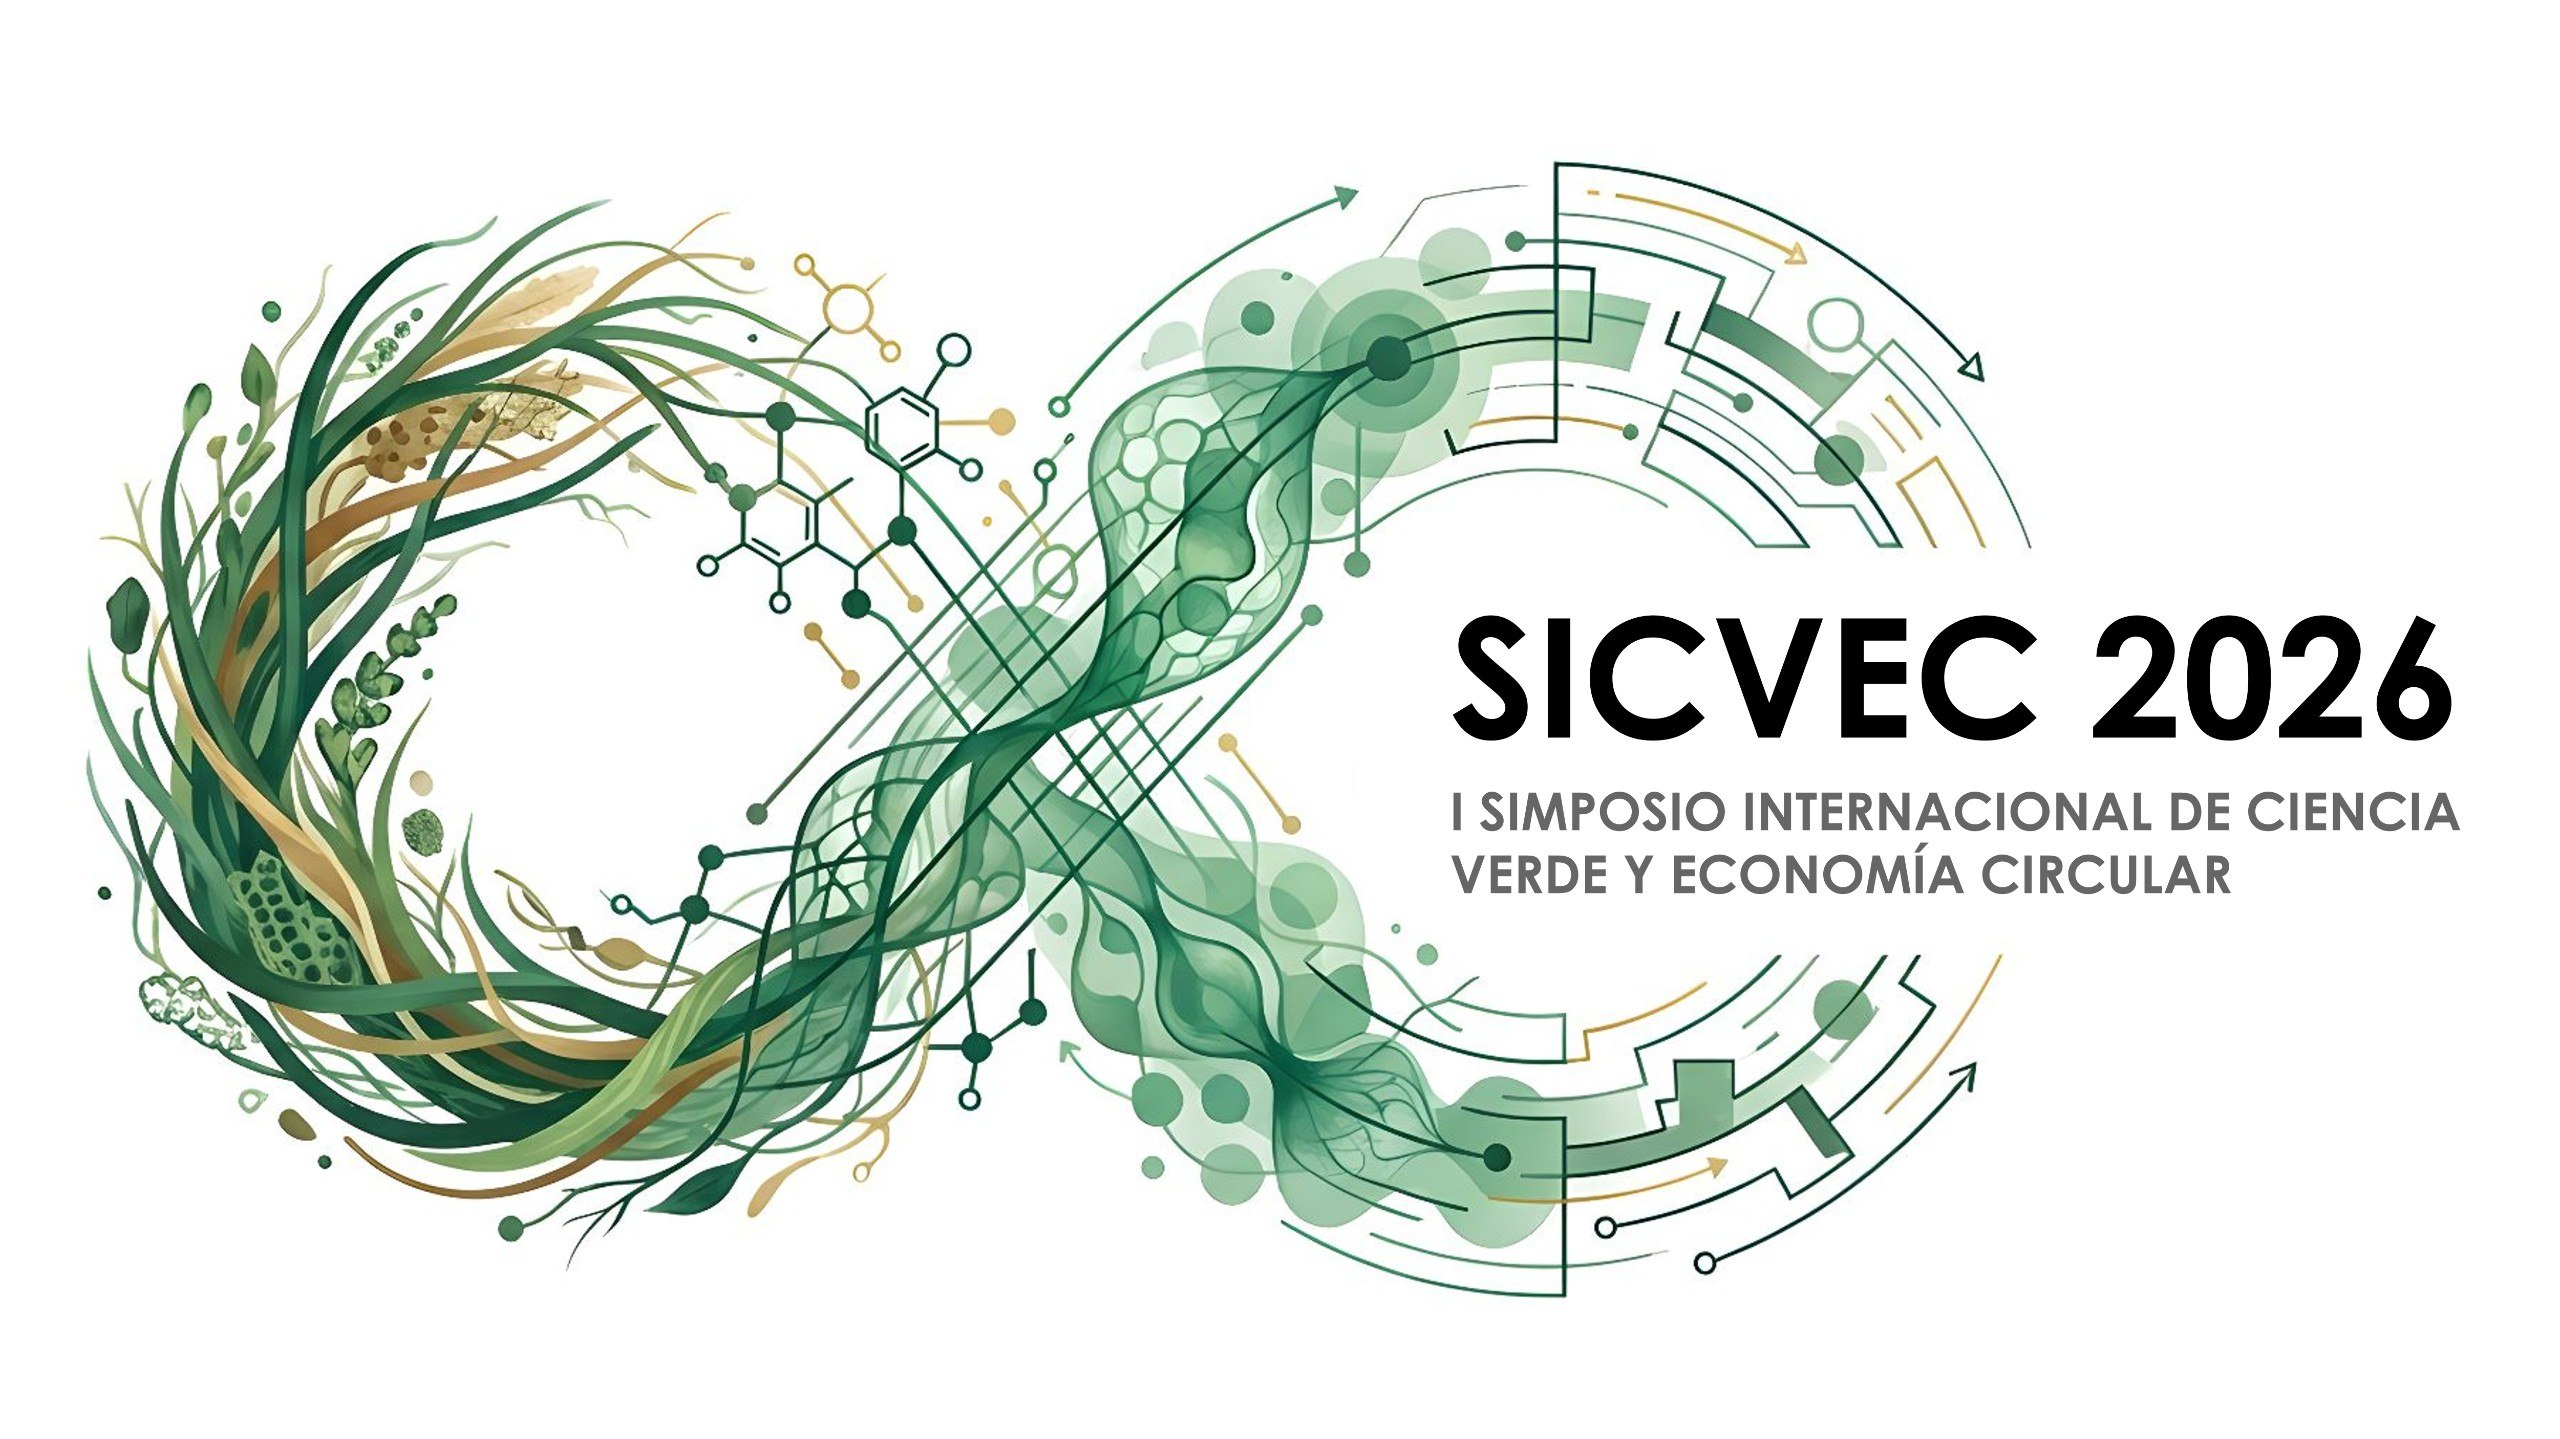
\includegraphics[height=0.8cm]{logo_sicvec2026.png} &
    
\includegraphics[height=0.8cm]{Logo_insilico.jpeg} \\
  \end{tabular*}%
}
\renewcommand{\headrulewidth}{1pt}
\renewcommand{\headrule}{\hbox to\headwidth{\color{verdeosc}\leaders\hrule height\headrulewidth\hfill}}

\begin{document}

\vspace{0.3cm}

\begin{center}
\textbf{\Large SIMPOSIO INTERNACIONAL DE CIENCIA VERDE Y ECONOMÍA CIRCULAR}

\textbf{\large SICVEC 2026}

\textit{Información para Conferencistas Invitados}
\end{center}

\vspace{0.3cm}

\noindent
\textbf{EVENTO}

\begin{tabular}{ll}
\textbf{Nombre:} & Simposio Internacional de Ciencia Verde y Economía Circular 2026 \\
\textbf{Fechas:} & 19 y 20 de octubre de 2026 (lunes y martes) \\
\textbf{Lugar:} & Centro Comercial Guacarí, Sincelejo, Sucre, Colombia \\
\textbf{Modalidad:} & Híbrida (presencial + virtual en línea) \\
\textbf{Participantes:} & 120–150 asistentes presenciales + 100 cupos virtuales \\
\end{tabular}

\vspace{0.3cm}

\noindent
\textbf{EJES TEMÁTICOS}

\begin{enumerate}\setlength{\itemsep}{0.15cm}
\item Economía Circular y Procesos Lineales
\item Química Verde y Procesos Sostenibles
\item Biotecnología Sostenible
\item Tecnologías Verdes y Energías Renovables
\item Sostenibilidad en Cadenas de Suministro
\item Política Pública y Gobernanza Ambiental
\end{enumerate}

\vspace{0.2cm}

\noindent
\textbf{CONFERENCIAS MAGISTRALES}

Duración: 45 minutos de presentación + 15 minutos de preguntas y discusión.

Formato: Virtual (en línea). Invitación académica.

Distribución: Dos conferencistas por día (mañana y tarde).

\vspace{0.2cm}

\noindent
\textbf{CRONOGRAMA DEL EVENTO}

\begin{tabular}{lll}
\textbf{Actividad} & \textbf{Fecha} & \textbf{Hora} \\
\hline
Cierre convocatoria trabajos & 28 sept 2026 & 23:59 (hora Colombia) \\
Notificación aceptación & 6 octubre 2026 & — \\
Envío de materiales finales & 14 octubre 2026 & — \\
\textbf{Simposio SICVEC 2026} & \textbf{19–20 octubre 2026} & \textbf{08:00–18:00} \\
Publicación de memorias & 20 octubre 2026 & — \\
\end{tabular}

\vspace{0.2cm}

\noindent
\textbf{REQUISITOS PARA CONFERENCISTAS}

\begin{enumerate}\setlength{\itemsep}{0.15cm}
\item Confirmar disponibilidad antes del 25 de septiembre (20 de septiembre para ponentes internacionales)
\item Proponer título y resumen de la conferencia
\item Proporcionar biografía actualizada y foto de perfil (para promoción)
\item Confirmar detalles técnicos antes del 1 de octubre
\end{enumerate}

\vspace{0.2cm}

\noindent
\textbf{ORGANIZADORES Y CONTACTO}

\textbf{Coordinación General:} Dr. Aldo F. Combariza Montañez
\textit{Grupo de Investigación IN SILICO, Universidad de Sucre}
Email: \href{mailto:aldo.combariza@unisucre.edu.co}{aldo.combariza@unisucre.edu.co}

\vspace{0.2cm}

\noindent
\rule{\textwidth}{0.5pt}

\vspace{0.2cm}

\noindent
\textit{\small SICVEC 2026 contribuye a los Objetivos de Desarrollo Sostenible: ODS 12 (Consumo responsable), ODS 13 (Acción climática), ODS 15 (Vida terrestre), ODS 17 (Alianzas).}

\end{document}
